\documentclass[a4paper,oneside]{report}
\usepackage{pgfplots}
\ifx\HCode\UnDef\else\def\pgfsysdriver{pgfsys-tex4ht.def}\fi
\usepackage{verbatim}
\usepackage{listings}
\usepackage{tikz,graphicx}
\usepackage{caption}
\usepackage{float}
\usepackage{hyperref}
\usepackage{subfiles}
\usepackage{nomencl}
\usepackage{chngcntr}
\makenomenclature

\usepackage{makeidx}
\makeindex

\counterwithout{figure}{chapter}

\usetikzlibrary{external,calc,trees,positioning,arrows,chains,shapes.geometric,%
decorations.pathreplacing,decorations.pathmorphing,shapes,%
matrix,fit,shapes.symbols,backgrounds,fit}
\captionsetup[figure]{labelformat=simple}

\renewcommand{\figurename}{Figure}
% Returns three nodes: The argument, and the projections of the argument on the left and right borders of the bounding box
\newcommand{\extendnode}[1]{
    (#1)
    ($(current bounding box.north east)!(#1)!(current bounding box.south east)$)
    ($(current bounding box.north west)!(#1)!(current bounding box.south west)$)
}

\usetikzlibrary{calc,trees,positioning,arrows,chains,shapes.geometric,%
decorations.pathreplacing,decorations.pathmorphing,shapes,%
matrix,shapes.symbols,backgrounds,fit,intersections}

\title{OAI EPC current development}
\author{Sebastien ROUX\\Eurecom\\sebastien.roux@eurecom.fr}

\definecolor{javared}{rgb}{0.6,0,0} % for strings
\definecolor{javagreen}{rgb}{0.25,0.5,0.35} % comments
\definecolor{ckeyw}{rgb}{0,0,0.8} % keywords
\definecolor{ccomment}{rgb}{0.6,0.6,0.6} % javadoc

\lstset{
    language=C,
    basicstyle=\ttfamily,
    keywordstyle=\color{ckeyw}\bfseries,
    stringstyle=\color{javared},
    commentstyle=\color{ccomment},
    morecomment=[s][\color{ccomment}]{/**}{*/},
    numbers=left,
    numberstyle=\tiny\color{black},
    stepnumber=1,
    numbersep=10pt,
    tabsize=4,
    showspaces=false,
    showstringspaces=false,
    breaklines
}


\tikzset{
    table nodes/.style={
        rectangle,
        rounded corners=0.6mm,
        draw=black,
        align=center,
        minimum height=7mm,
        minimum width=22mm,
        text depth=0.5ex,
        text height=2ex,
        %         inner xsep=0pt,
        outer sep=0pt,
    },
    table/.style={
        matrix of nodes,
        %         row sep=-\pgflinewidth,
        %         column sep=-\pgflinewidth,
        rectangle,
        nodes={
            table nodes
        },
        execute at empty cell={\node[draw=none]{};}
    },
    cps/.style={
        draw=black,
        fill=blue!20,
        rounded corners=0.6mm,
    },
    ups/.style={
        draw=black,
        fill=yellow!30,
        rounded corners=0.6mm,
    },
    stdlinux/.style={
        draw=black,
        fill=green!10,
        rounded corners=0.6mm,
    },
    rect/.style={
        rectangle,
        draw,
    },
    schritt/.style={
        draw,
        rounded corners,
        fill=blue!20,
        inner xsep=2em,
    },
    t0/.style={draw,fill=blue!20},
    t1/.style={draw,fill=blue!40},
    background/.style={
        draw,
        fill=yellow!30,
        align=center,
        dashed,
    },
    background2/.style={
        draw,
        fill=green!15,
        align=center,
    },
    connector/.style={
        -latex,
        font=\scriptsize
    },
    rectangle connector/.style={
        connector,
        to path={(\tikztostart) -| (\tikztotarget) },
        pos=0.5
    },
    rectangle connector/.default=-2cm,
    straight connector/.style={
        connector,
        to path=--(\tikztotarget) \tikztonodes
    },
    queue/.style={
        draw,
        fill=yellow!30,
        cylinder,
        aspect=0.7,
        minimum height=1cm,
        minimum width=0.7cm
    },
}
\renewcommand{\nomname}{List of Abbreviations}
\renewcommand{\thefigure}{\Alph{figure}}

\begin{document}
\maketitle
\tableofcontents
\printnomenclature[2cm]

\chapter*{MME and S+P-Gateway} \stepcounter{chapter}
\addcontentsline{toc}{chapter}{MME and S+P-Gateway}

% \nomenclature{MME}{Mobility Management Entity}
% \nomenclature{S-GW}{Serving Gateway}
% \nomenclature{P-GW}{PDN Gateway}
\begin{figure}[H]
\begin{center}
\begin{tikzpicture}
\tikzstyle{every node}=[font=\footnotesize]
\matrix (table) [row sep=0.5cm, column sep={3.2cm,between origins}, table,text width=3mm,name=table] {
    & & &\\
    & & &\\
    & & &\\
    & & &\\
    & & &\\
};
\node(MMEAPP)[cps,draw,fit=(table-1-1)(table-1-2),table nodes]{MME Application};
\node(SPGW)[cps,draw,fit=(table-1-3)(table-1-4),table nodes]{S+P-GW Application};
\node(NAS)[cps,draw,fit=(table-2-2),table nodes]{NAS};
\node(S6A)[dashed,cps,draw,fit=(table-3-1),table nodes]{S6a/Diameter};
\node(S1AP)[cps,draw,fit=(table-3-2),table nodes]{S1-MME/S1AP};
\node(S1U)[ups,draw,fit=(table-3-3),table nodes]{S1-U/GTPU};
\node(SGI)[dashed,ups,draw,fit=(table-3-4),table nodes]{SGi};
\node(SCTP)[stdlinux,draw,fit=(table-4-1)(table-4-2),table nodes]{SCTP};
\node(UDP)[stdlinux,draw,fit=(table-4-3),table nodes]{UDP};
\node(IP)[stdlinux,draw,fit=(table-5-1)(table-5-2)(table-5-3)(table-5-4),table nodes]{IP};

\draw[<->, dashed, draw=red] (MMEAPP) -- node(arrow1)[above, align=center]{S11}(SPGW);
\draw[<-,dashed] (S1U) -- (SPGW.south-|S1U);
\draw[<-,dashed] (SGI) -- (SPGW.south-|SGI);
\draw[-] (S6A) -- (MMEAPP.south-|S6A);
\draw[-] (NAS) -- (MMEAPP.south-|NAS);
\draw[-] (S1AP) -- (NAS);
\draw[-] (S1U) -- (SGI);
\draw[-] (S1U) -- (UDP);
\draw[-] (S1AP) -- (SCTP.north-|S1AP);
\draw[-] (S6A) -- (SCTP.north-|S6A);
\draw[-] (SCTP) -- (IP.north-|SCTP);
\draw[-] (UDP) -- (IP.north-|UDP);
\draw[-] (SGI) -- (IP.north-|SGI);
\draw[-] (MMEAPP.south) |- (S1AP.west);

\draw($(table.north west) + (-2mm,1mm)$) rectangle ($(table.south east) + (2mm,-1mm)$);

\node[cps, minimum width=5mm,minimum height=5mm,below=of IP.south west,anchor=west](l1){};
\node[right=2mm of l1](ct1) {Control Plane};
\node[ups,minimum width=5mm,minimum height=5mm,below=0.3cm of l1](l2){};
\node[below=0.3cm of ct1, right=2mm of l2](ct2) {User Plane};
\node[stdlinux,minimum width=5mm,minimum height=5mm,below=0.3cm of l2](l3){};
\node[below=0.3cm of ct2, right=2mm of l3](ct3) {Linux IP Stack};
\draw[minimum width=5mm,minimum height=5mm,below=0.3cm of l3,<->,dashed, draw=red]
($(l3.south west) - (0,0.55cm)$) -- node(l4){} ($(l3.south east) - (0,0.55cm)$);
\node[right=2mm of l4.north east](ct4) {Abstraction link};
\draw[minimum width=5mm,minimum height=5mm,below=0.3cm of l4,->,dashed]
($(l4.south west) - (0,0.25cm)$) -- node(l5){} ($(l4.south east) - (0,0.25cm)$);
\node[right=2mm of l5.north east](ct5) {Control};
\node[draw,fit=(ct1)(l1)(ct2)(l2)(ct3)(l3)(ct4)(l4)(ct5)(l5)] {};

\end{tikzpicture}
\caption{MME and S+P-GW architecture} \label{fig:MMEoverall}
\end{center}
\end{figure}

Figure \ref{fig:MMEoverall} shows the targeted implementation of Eurecom
EPC.

\chapter*{S1AP layer} \stepcounter{chapter}
\addcontentsline{toc}{chapter}{S1AP layer}

\nomenclature{S1AP}{S1 Application Protocol}S1AP layer relies on
\nomenclature{ASN.1}{Abstract Syntax Notation.1}ASN.1 messages
description. Generating C code from the specification
implies three steps:
\begin{enumerate}
\item Modify .asn files to match tools limitation.
\item Generate \nomenclature{IE}{Informations Elements}IEs with the help of the asn1c free tool.
\item Use the provided script which generates \nomenclature{PDU}{Protocol Data Unit}PDU codec\footnote{Encode/Decode}.
\end{enumerate}

\chapter*{Inter-task interface} \stepcounter{chapter}
\addcontentsline{toc}{chapter}{Inter-task interface}

\section{Concurrency}

Code divided in layers should be able to be executed in parallel to use the full
\nomenclature{CPU}{Control Processing Unit}CPUs power. We can achieve better performance
by using some mechanisms that runs part of code in parallel on UNIX platforms:
\begin{itemize}
\item Multi-process: no link between processes, usage of sockets or pipes is mandatory.
\item Forks: code is duplicated and data are stored in different spaces.
\item Threads: only code is duplicated, data space is shared between processes
\end{itemize}
Data synchronization is the first issue to think about when using such mechanisms.

\section{Overall description}

A single \nomenclature{API}{Application Programming Interface}API
(called ITTI\footnote{InTer-Task Interface}) is used to manage messages
exchanged between the tasks which are running on separate threads.
This will lead in better usage of multi-core environments.
\begin{figure}[h]
    \begin{center}
    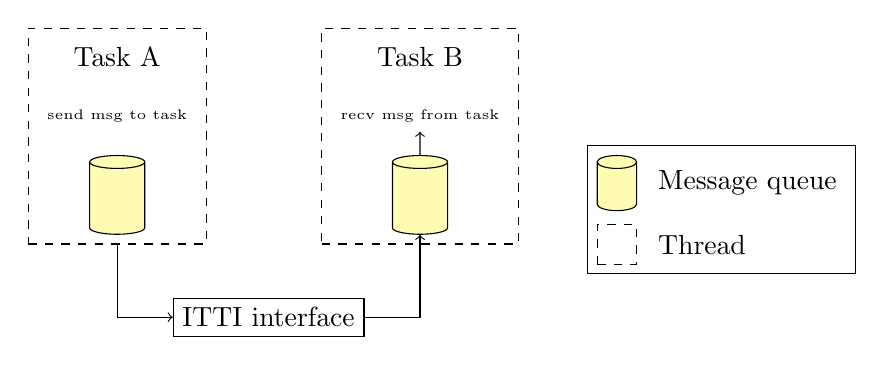
\begin{tikzpicture}
        \node[](t1) { Task A };
        \node[below=of t1,yshift=7mm,font=\tiny](s1) { send msg to task };
        \node[queue,rotate=90,below=of t1.south,anchor=top](c1) {};
        \node[right=of t1,xshift=15mm](t2) { Task B };
        \node[below=of t2,yshift=7mm,font=\tiny](r2) { recv msg from task };
        \node[queue,rotate=90,below=of t2.south,anchor=top](c2) {};
        \node[dashed,fit=(c1)(t1)(s1),draw](T1){};
        \node[dashed,fit=(c2)(t2)(r2),draw](T2){};
        \node[draw](ITTI) at ($(T1)!0.5!(T2) + (0, -2.3)$){ITTI interface};
        \draw[->] (T1) |- (ITTI);
        \draw[->] (ITTI.east) -| (c2.bottom);
        \draw[->] (c2.east) -- (r2);
        \node[queue,rotate=90,minimum width=5mm,minimum height=7mm,right=of c2,anchor=top,yshift=-15mm](c3) {};
        \node[dashed,rectangle,minimum width=5mm,minimum height=5mm,draw,below=7mm of c3,anchor=east](c4) {};
        \node[right=4mm of c3.shape center](x3){Message queue};
        \node[right=4mm of c4.center](x4){Thread};
        \node[draw,fit=(c3)(x3)(x4)(c4)](T4){};
    \end{tikzpicture}
    \caption{Overall process} \label{fig:Overall process}
    \end{center}
\end{figure}
Figure \ref{fig:Overall process} describes the basic fonctionnement of the inter-task interface.
A message sent from
Task A is en-queued to the message queue belonging to the target task. Note that
tasks can send messages to themselves. Another API (See Figure \ref{fig:Broadcasting process}) defines broadcast messaging
where any task can send a broadcast message to every other task.
\begin{figure}[H]
    \begin{center}
    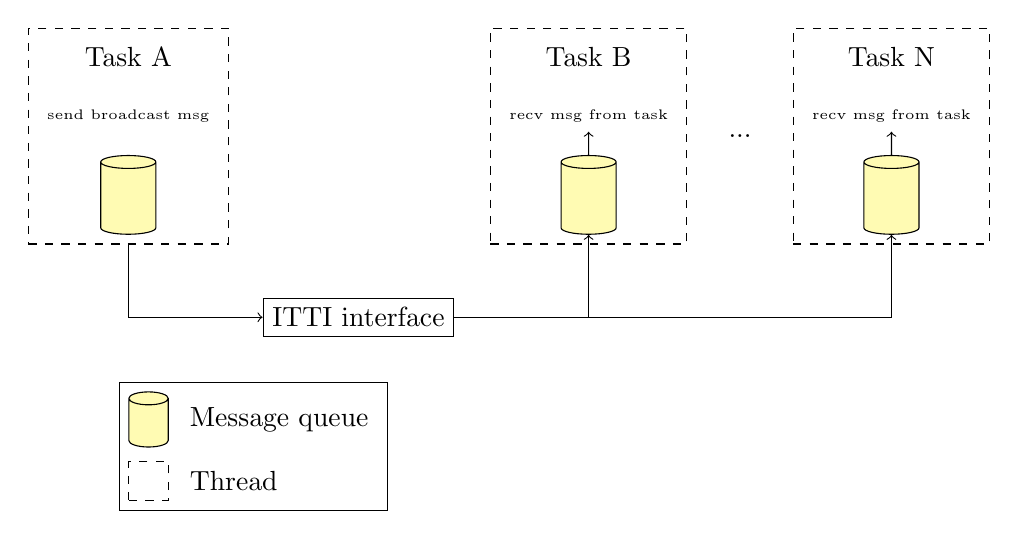
\begin{tikzpicture}
        \node[](t1) { Task A };
        \node[below=of t1,yshift=7mm,font=\tiny](s1) { send broadcast msg };
        \node[queue,rotate=90,below=of t1.south,anchor=top](c1) {};
        
        \node[right=of t1,xshift=35mm](t2) { Task B };
        \node[below=of t2,yshift=7mm,font=\tiny](r2) { recv msg from task };
        \node[queue,rotate=90,below=of t2.south,anchor=top](c2) {};
        
        \node[right=of t2,xshift=15mm](tn) { Task N };
        \node[below=of tn,yshift=7mm,font=\tiny](rn) { recv msg from task };
        \node[queue,rotate=90,below=of tn.south,anchor=top](cn) {};
        \node[dashed,fit=(c1)(t1)(s1),draw](T1){};
        \node[dashed,fit=(c2)(t2)(r2),draw](T2){};
        \node[dashed,fit=(cn)(tn)(rn),draw](TN){};

        \node[](ITTI) at ($(T2)!0.5!(TN)$){...};
        \node[draw](ITTI) at ($(T1)!0.5!(T2) + (0, -2.3)$){ITTI interface};
        \draw[->] (T1) |- (ITTI);
        \draw[->] (ITTI.east) -| (c2.bottom);
        \draw[->] (ITTI.east) -| (cn.bottom);
        \draw[->] (c2.east) -- (r2);
        \draw[->] (cn.east) -- (rn);
	\node[queue,rotate=90,minimum width=5mm,minimum height=7mm,below=23mm of T1](c3) {};
	\node[dashed,rectangle,minimum width=5mm,minimum height=5mm,draw,below=7mm of c3,anchor=east](c4) {};
	\node[right=4mm of c3.shape center](x3){Message queue};
	\node[right=4mm of c4.center](x4){Thread};
	\node[draw,fit=(c3)(x3)(x4)(c4)](T4){};
    \end{tikzpicture}
    \caption{Broadcasting process} \label{fig:Broadcasting process}
    \end{center}
\end{figure}
Once a task received a new message and if the task is in sleep mode (i.e. not handling
any message), the task is waken up and the message is de-queued. We can imagine a limit
in number of parallel tasks, for example N+1 CPU's. Architectures using hyper-threading
mechanism can have this value extended to 2 x CPU's.
Every task is running in a separated pthread, awaiting for new messages to handle.

\section{Signals from kernel}

Handling of signals from kernel is the more critical part as a signal can be raised
at any moment and will interrupt one of the running thread. Used signals should be restricted 
to a single task that will handle them (using the POSIX sigmask function) . Moreover, it isn't
thread-safe to use mutexes inside a signal handler, a synchronization flag should be used to
notify the signal handler task. This task will then send the appropriate message
to the right task. For example, handling of signals can be done in the main thread or by a background task
scheduled periodically.
To overcome these issues, sigtimedwait and sigwaitinfo API functions can be used
to wait for a signal to happen. Signals will be received in the thread context, as far as
other threads block these signals.

\section{Priority handling}

Usage of message prioritization enables tasks to send critical messages with a faster
delivery time regarding other messages en-queued for the target task.
For now only seven priority levels can be applied when defining tasks:
\begin{itemize}
\item TASK\_PRIORITY\_MAX
\item TASK\_PRIORITY\_MAX\_LEAST
\item TASK\_PRIORITY\_MED\_PLUS
\item TASK\_PRIORITY\_MED
\item TASK\_PRIORITY\_MED\_LEAST
\item TASK\_PRIORITY\_MIN\_PLUS
\item TASK\_PRIORITY\_MIN
\end{itemize}
For now message priority does not involve any suitable scheduler: every time a message is de-queued,
message priority of other messages is incremented by one.

\section{Message scheduling}
Currently, there is no software limit on the maximum number of threads executed in parallel.
When a task sends a message, it is en-queued in the right message queue, belonging to
the target task. The queue is a double-linked list. A mutex prevents other tasks
from modifying this queue while a task is en-queueing or removing a message.

\section{Message definition}
Messages are defined using a single macro that adds the message to the ids enumeration
and maps data of the message to the union of messages.
\begin{lstlisting}
MESSAGE_DEF(S1AP_SCTP_NEW_MESSAGE_IND,    TASK_PRIORITY_MED, S1apSctpNewMessageInd s1apSctpNewMessageInd)
\end{lstlisting}
and the associated data:
\begin{lstlisting}
typedef struct {
    uint8_t  *buffer;     ///< SCTP buffer
    uint32_t  bufLen;     ///< SCTP buffer length
    int32_t   assocId;    ///< SCTP physical association ID
    uint8_t   stream;     ///< Stream number on which data had been received
    uint16_t  instreams;  ///< Number of input streams for the SCTP connection between peers
    uint16_t  outstreams; ///< Number of output streams for the SCTP connection between peers
} S1apSctpNewMessageInd;
\end{lstlisting}
\section{Task message handling}
\begin{lstlisting}
void* s1ap_mme_thread(void *args) {
    while(1) {
        /* Trying to fetch a message from the message queue.
         * If the queue is empty, this function will block till a
         * message is sent to the task.
         */
        receive_msg(TASK_S1AP, &receivedMessage);
        assert(receivedMessage != NULL);
        switch(receivedMessage->messageId) {
            case S1AP_SCTP_NEW_MESSAGE_IND:
            {
                //Some processing
            } break;
            default:
            {
                S1AP_DEBUG("Unkwnon message ID %d\n", receivedMessage->messageId);
            } break;
        }
        free(receivedMessage);
        receivedMessage = NULL;
    }
    return NULL;
}
\end{lstlisting}
\section{Messages logging}
\begin{figure}[H]
    \begin{center}
    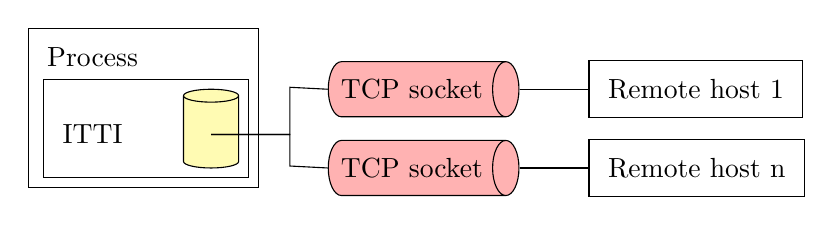
\begin{tikzpicture}
    \node[](p1) { Process };
    \node[below=5mm of p1](i1) { ITTI };
    \node[queue,right=of i1,rotate=90,anchor=base](q1) {};
    \node[draw,fit=(i1)(q1)](s1) {  };
    \node[fit=(p1)(i1)(q1)(s1),draw](T1){};
    \node[queue,fill=red!30,right=of s1.east,yshift=-5mm](c1) { TCP socket };
    \node[right=of c1](r1){ Remote host n };
    \node[fit=(r1),draw](R2){};
    \node[queue,fill=red!30,right=of s1.east,yshift=5mm](c2) { TCP socket };
    \node[right=of c2](r1){ Remote host 1 };
    \node[fit=(r1),draw](R1){};
    \draw[-] (q1.base) -- ++ (1,0) -| ++ (0,.6) -- (c2.west);
    \draw[-] (c2) -- (R1);
    \draw[-] (q1.base) -- ++ (1,0) -| ++ (0,-.4) -- (c1.west);
    \draw[-] (c1) -- (R2);
    \end{tikzpicture}
    \caption{Remote debugging} \label{fig:Remote debugging}
    \end{center}
\end{figure}
Logging of inter-tasks messages can be setup using an external tool that will be
connected to the ITTI. Based on an array of dumped messages, they are serialized
to produce an array of byte sent over a socket. A remote tool can then decode
messages and display fields, message number, time.\\
Additionaly, logs from standard output can be printed over the debug tool.
Multi-user debugging on only one running process can be achieved using this interface.
Messages to dump should be queued for a pure asynchronous communication between the
dump task and the remote hosts.
Another interesting feature could be to send a message to a task from an host,
allowing run-time re-configuration.
The C pre-processor can be used to generate messages definition (using
\nomenclature{XML}{Extensible Markup Language}XML templates
for example).\\
\section{Limitations}
Data pointers belonging to one task should never be passed to another task.
The presented mechanism does not prevent a task from being locked. In such a case,
the blocked task will no more handle messages incoming from other tasks.

\section{Benefits}
\begin{itemize}
 \item Only a single entry point between all tasks (easy inter-task communication tracking and debugging).
 \item Usage of message queues enables parallelization of layers.
 \item Message prioritization and scheduling.
 \item Protection of data between threads is done by the API at an higher level.
\end{itemize}

\section{To do}
\begin{itemize}
 \item Implement a priority based scheduler. Currently the queue of messages works as a FIFO.
 \item Limit the number of tasks thread that can be run in parallel
\end{itemize}

\chapter*{Signal API} \stepcounter{chapter}
\addcontentsline{toc}{chapter}{Signal API}

On LINUX platforms, processes will receive signals comming from Kernel.
A single blocking entry point handles all used signals that are requested by the
MME. The main application thread is reserved to signal handling as this thread will
be blocked till a new signal is ready for handling.\\
Using this method prevents threads from being interrupted by signals handler which
can interrupt the thread at any time and as a consequence create some misbehaving
in threads contexts.
Following is a sample list of signals handled:
\begin{itemize}
 \item SIGABRT This is signal is sent to the process when abort() function is called
 within the process and kill the process. Process can for example display the stack
 once this signal is received.
 \item SIGRTMIN This signal is used by the timer API and is raised everytime a
 timer has expired.
\end{itemize}
Till now there is no way for tasks to request a new signal.

\chapter*{Timer API} \stepcounter{chapter}
\addcontentsline{toc}{chapter}{Timer API}

Timer API doesn't consist of a task (i.e. tasks cannot send messages to it).
Handling of UNIX signal associated to the timers is a Real-time signal with an id (SIGRTMIN)
depending on the platform. Management of this signal is done by the signal interface
and developpers should not care about handling timer signals incoming from Kernel.
Once a timer has expired the task which has requested it will receive the TIMER\_HAS\_EXPIRED
signal.
Note that timer\_id is of type long and thus its size is platform specific.

\section{Timer types}

\begin{itemize}
 \item TIMER\_ONE\_SHOT After expiry and its associated signal, the timer is removed.
 \item TIMER\_PERIODIC The timer is automatically reloaded on each expiry while the task
which has setup this timer doesn't cancel it.
\end{itemize}

\section{Requesting a new signal}
Any task can request a new signal by invoking the following API:
\begin{lstlisting}
int timer_setup(
    uint32_t      interval_sec,
    uint32_t      interval_us,
    task_id_t     task_id,
    timer_type_t  type,
    long         *timer_id);
\end{lstlisting}

Note that timer id is a unique identifier to distinguish timers.

\section{Disable and remove a timer}

Disable and remove the timer referenced by timer\_id.
\begin{lstlisting}
int timer_remove(long timer_id);
\end{lstlisting}

\section{Timer signal expiry}

Once the signal dispatcher receives the SIGRTMIN signal, a new signal is sent
to the task which has requested the timer. Contrary to signal request, timer
expiry notification is achieved using the intertask mechanism.
The signal data associated to this event follows:
\begin{lstlisting}
typedef struct {
    long timer_id;
} timer_has_expired_t;
\end{lstlisting}

\chapter*{Compiling core EPC} \stepcounter{chapter}
\addcontentsline{toc}{chapter}{Compiling core EPC}

The core EPC software has been tested on Ubuntu 12.04LTS x86 and ia64.
Before compiling the core EPC, some packages should be installed on the platform.

\section{Dependencies}

\begin{itemize}
 \item libsctp-dev
 \item libpthread-dev
 \item automake and autoconf
 \item libtoolize
 \item gcc, g++, make
 \item flex and bison
 \item openssl-dev
 \item asn1c (see section \ref{sec:asn1c})
 \item freediameter (see section \ref{sec:freediameter}) and gnutls 3.1.0
 (see section \ref{sec:gnutls})
\end{itemize}
Command-line to install the required packages:
\begin{lstlisting}
sudo apt-get install cmake make gcc flex bison \
libsctp1 libsctp-dev libidn2-0-dev libidn11-dev \
libmysqlclient-dev libxml2-dev swig python-dev \
cmake-curses-gui valgrind guile-2.0-dev \
libgmp-dev libgcrypt11-dev gdb unzip \
libtasn1-3-dev g++ autoconf automake \
openssl-dev -y
\end{lstlisting}

\subsection{ASN1c}
\label{sec:asn1c}

\subsection{gnutls}
\label{sec:gnutls}

The GNUTls library is only used by freediameter for certificate handling and as a
consequence should be installed before trying to compile the freediameter library.
\begin{lstlisting}
wget ftp://ftp.gnutls.org/gcrypt/gnutls/v3.1/gnutls-3.1.0.tar.xz
tar -xvf gnutls-3.1.0.tar.xz
cd gnutls-3.1.0/
./configure LDFLAGS='-L/usr/local/lib'
make
sudo make install
\end{lstlisting}
Note: when dependencies are installed in /usr/local instead of /usr,
LDFLAGS has to be overriden with the path to libraries when configuring the package:
LDFLAGS='-L/usr/local/lib'.

\subsection{freediameter}
\label{sec:freediameter}
Freediameter is the package that provides diameter capabilities to the MME/HSS.
On top of this stack, S6A avp dictionnary is used to enable a compliant S6A interface.
\begin{lstlisting}
wget http://www.freediameter.net/hg/freeDiameter/archive/1.1.5.tar.gz
tar -xvf 1.1.5.tar.gz
cd freeDiameter-1.1.5
patch -p1 < ../../freediameter-1.1.5.patch
mkdir build
cd build
cmake ../
make
make test
sudo make install
\end{lstlisting}
If you want ot install this package in /usr instead of /usr/local,\\
-DCMAKE\_INSTALL\_PREFIX:PATH=/usr should be passed to cmake at configuration.

\chapter*{System configuration} \stepcounter{chapter}
\addcontentsline{toc}{chapter}{System configuration}

Currently there is two ways to configure the system:
\begin{itemize}
 \item Compilation configuration
 \item Boot-up configuration
\end{itemize}
In the first type of configuration, the single system configuration structure
is filled in with default values that can be found in the mme\_default\_values.h
header file.\\
When Boot-up configuration is used, a configuration file is passed to the process
by using the either -c filename.conf or --conf=filename.conf. This file is then parsed
by the bison interpreter and values are replaced in the global system configuration
structure.

\section{Global MME parameters}

\subsection{Relative MME capacity}
Even though this parameter is not used by the MME for controlling the MME load
balancing within a pool (at least for now), the parameter has to be to forwarded
to the eNBs during association procedure.
This parameter is encoded on 8bits, acceptable values going from 0 to 255.
(Default value = 15)
\begin{lstlisting}
RELATIVE_CAPACITY = 10;
\end{lstlisting}

\subsection{Maximum number of UE}
\label{sec:Maximum number of UE}
This limit is present here only for debug purposes and is used to restrict
the number of served UE the MME can handle. In real network another mechanism
will trigger an MME overload for certain eNBs and will restrict certain types of
traffic. Such a mechanism would imply the Relative MME capacity.
\begin{lstlisting}
MAXUE = 100;
\end{lstlisting}

\subsection{Maximum number of eNB}
Refer to \ref{sec:Maximum number of UE}.
\begin{lstlisting}
MAXENB = 10;
\end{lstlisting}

\subsection{Tracking Area Identity}
\nomenclature{TAI}{Tracking Area Identity}TAI is the concatenation of
\nomenclature{MCC}{Mobile Country Code}MCC, \nomenclature{MNC}{Mobile Network Code}MNC and
\nomenclature{TAC}{Tracking Area Code}TAC.
The TAC uniquely identifies a PLMN within a Cell Id.
\begin{lstlisting}
PLMN = mcc.mnc:tac;
\end{lstlisting}
Multiple values can be given using a comma separator. Example:
\begin{lstlisting}
PLMN = 208.38:0,209.130:4,208.35:8;
\end{lstlisting}

\subsection{MME Code}
A list of a maximum of 256 values can be provided.
\nomenclature{MMEC}{MME Code}MME Code is encoded on 8 bits,
so acceptable range is: 0 to 255.
Example:
\begin{lstlisting}
MME_CODE = 30,56,1,8;
\end{lstlisting}

\subsection{MME Group Id}
A list of a maximum of 65356 values can be provided.
\nomenclature{MMEGID}{MME Group Id}MME Group Id is encoded on 16 bits,
so acceptable range is: 0 to 65535.
Example:
\begin{lstlisting}
MME_GID = 3,4,5,30,8,9,50021;
\end{lstlisting}

\section{Intertask parameters}
\subsection{Queue size per task}
To restrict the number of messages in queues or to detect a possible MME overload,
an upper bound for the queue size can be defined like this:
\begin{lstlisting}
ITTI_QUEUE_SIZE = 2000000;
\end{lstlisting}
This parameter is expressed in bytes. Note that all messages exchanged by tasks
have the same size.

\section{SCTP parameters}
\subsection{IN/OUT streams number}
The number of input/output streams can be configured to limit the number of streams
used for UE-associated signalling. Note that stream with id = 0 is reserved for
non-UE associated signalling. At least two streams should be used by the MME.
(Default value = 64/64 streams)
\begin{lstlisting}
SCTP_INSTREAMS = 32;
SCTP_OUTSTREAMS = 32;
\end{lstlisting}

\section{S1AP parameters}
\subsection{Outcome timer}
Once an outcome is sent from MME to eNB, the MME locally starts a timer to abort
the procedure and release UE contexts if the expected answer to this outcome is not
received at the expiry of this timer.\\
This timer is expressed in seconds. (Default value = 5 seconds)
\begin{lstlisting}
S1AP_OUTCOME_TIMER = 10;
\end{lstlisting}

\section{Network interfaces parameters}

Three paramters can be tuned in the configuration file:
\begin{itemize}
 \item Interface Name: The related interface will be bind to this interface name
 \item IP address: Currently only IPv4 address is allowed
 \item IP netwmask: Netmask for the LAN
\end{itemize}
These three paramters can be setup for five different interfaces used:
\begin{itemize}
 \item SGW interface for S11
 \item SGW interface for S1U/S12/S4 in user plane
 \item SGW interface for S5/S8 in user plane
 \item PGW interface for S5/S8
 \item PGW interface for SGi
 \item MME interface for S1-MME in control plane
\end{itemize}
Example of configuration:
\begin{lstlisting}
# ------- Interfaces definitions
SGW_INTERFACE_NAME_FOR_S11            = "s11sgw";
SGW_IP_ADDRESS_FOR_S11                = "192.168.10.1";
SGW_IP_NETMASK_FOR_S11                = 24;

SGW_INTERFACE_NAME_FOR_S1U_S12_S4_UP  = "upsgw0";
SGW_IP_ADDRESS_FOR_S1U_S12_S4_UP      = "192.168.1.1";
SGW_IP_NETMASK_FOR_S1U_S12_S4_UP      = 24;

SGW_INTERFACE_NAME_FOR_S5_S8_UP       = "upsgw1";
SGW_IP_ADDRESS_FOR_S5_S8_UP           = "192.168.5.2";
SGW_IP_NETMASK_FOR_S5_S8_UP           = 24;

PGW_INTERFACE_NAME_FOR_S5_S8          = "uppgw0";
PGW_IP_ADDRESS_FOR_S5_S8              = "192.168.5.1";
PGW_IP_NETMASK_FOR_S5_S8              = 24;

PGW_INTERFACE_NAME_FOR_SGI            = "eth1";
PGW_IP_ADDR_FOR_SGI                   = "192.168.12.30";
PGW_IP_NETMASK_FOR_SGI                = 24;

MME_INTERFACE_NAME_FOR_S1_MME         = "cpmme0";
MME_IP_ADDRESS_FOR_S1_MME             = "192.168.11.1";
MME_IP_NETMASK_FOR_S1_MME             = 24;
\end{lstlisting}

\end{document}
